\documentclass[12pt]{article}
\usepackage{graphicx}
\usepackage{amsmath}

\begin{document}
\title{Stochastic Basics}
\author{Steven Wang}
\date{\today}
\maketitle

\tableofcontents

\section{Measure Theory Concepts}
\subsection{Banach Space}
Banach Space: A complete normed vector space.
$$\lim_{n\to\infty}x_n=x$$
$$\lim_{n\to\infty}||x_n-x||_x=0$$
A normed space $X$ is a Banach space if and only if each absolutely convergent series in X converges:
$$\sum_{n=1}^\infty||v_n||_X<\infty \Rightarrow \sum_{n=1}^\infty v_n\ converges\ in\ X$$


\subsection{$L^p$ Space}
$L^p$ Space: uncountable infinite dimension
$$(S,\Sigma,\mu)\quad L^p(S,\mu)=\{f; ||f||_p=(\int_S|f|^p d\mu)^{\frac{1}{p}}<\infty\}$$
$$||(x_n)_{n\in N}||_p=(|x_1|^p+|x_2|^p+...+|x_n|^p+...)=(\sum_{n\in N}|x_n|^p)^{\frac{1}{p}}$$
\indent The series on the right of the above euqation converges.
\\
\indent $L^p$ space is the subset of all the sequences whose elements make the series on the right of above equation converge.
\\
$$if\ p<q,then\ L^p<L^q,\quad this\ is\ a\ proper\ subset.$$
\begin{itemize}
    \item All $L^p$ spaces are Banach space.
    \item If and only if $p=2$, $L^2$ is Hilbert space.(???)
\end{itemize}
\\
Norm: A function that assigns a strictly positive length or size to each vector in a vector space, except 0 for zero vector:
\begin{enumerate}
    \item zero vector: $l(v)=0\Leftrightarrow v=0$
    \item linear: $\forall\lambda\in R, l(\lambda v)=\lambda l(v)$
    \item triangle inequality: $l(u)+l(v)\geq l(u+v)$
\end{enumerate}
\indent length function: $[\sum(X_i)^p]^{\frac{1}{p}}$


\subsection{Hilbert Space}
Hilbert Space:
\begin{itemize}
    \item It extends the methods of vector algebra and calculus from 2-dimension or 3-dimension to finite or infinite number of dimensions.
    \item A Hilbert space is an abstract vector space possessing the structure of an inner product that allows length and angle to be measured.
    \item As a complete normed space, Hilbert spaces are by definition also Banach spaces.
\end{itemize}



\subsection{$L^2$ Space}
$L^2$ Space: Countable infinite dimension. 所有平方收敛级数数列构成的空间(可数无限维)

\subsection{Some Notations}
\begin{itemize}
    \item $lim\ sup$: limit superior
    \item $lim\ inf$: limit inferior
    \item $inf$: infimum, greatest lower bound(GLB)
    \item $sup$: supremum, least upper bound(LUB)
\end{itemize}

$$\lim_{n\to\infty}sup\ x_n=b\quad\Rightarrow\quad There\ exists\ N, \epsilon\in R^+,\ x_n < b+\epsilon, \forall n>N$$
$$\lim_{n\to\infty}inf\ x_n=b\quad\Rightarrow\quad There\ exists\ N, \epsilon\in R^+,\ x_n > b-\epsilon, \forall n>N$$


\section{Ito Calculus}
Wiener Process: $W_t$\\
(or Brownian Process: $B_t$)\\
\\
Quadratic Variation: $(dW_t)^2=dt$\\
-A monotone increasing or decreasing function has bounded variation.\\
-A function with a continuous derivative has bounded variation.\\
-Wiener process does not have bounded variation.\\
-Wiener process has quadratic variation.\\
$$lim_{n\rightarrow\infty}E[\sum_{k=1}^n (W(\frac{kt}{n})-W(\frac{(k-1)t}{n}))^2]=t$$
Rough proof:
$$Z_{nk}=\frac{W(\frac{kt}{n})-W(\frac{(k-1)t}{n})}{\sqrt{t/n}}$$
$Z_{nk}$ is just a random variable with distribution $N(0,1)$.
$$\sum_{k=1}^n (W(\frac{kt}{n})-W(\frac{(k-1)t}{n}))^2=\sum_{k=1}^{n}\frac{t}{n}Z_{nk}^2=t(\frac{1}{n}\sum_{k=1}^{n}Z_{nk}^2)$$
whose expectation is the same thing as calculating the variance of the distribution $N(0,1)$.

\subsection{Ito's Lemma $f(B_t)$}
$$df=f'(B_t)dB_t + \frac{1}{2}f''(B_t)dt$$
%Check wikipedia
%Check for expression of 
$$df(t,X_t)=f_t dt + f_x dX_t+\frac{1}{2}f_{xx}d[X]_t$$
For normal calculus, we only have the first term.\\
The second term here is because of Quadratic Variation.\\
\\
For $f(t,x)$:\\
% Equation too long for one line
\begin{multline*}
f(t+\Delta t,x+\Delta x)=f(t,x)+\frac{\partial f(t,x)}{\partial t}\Delta t+\frac{\partial f(t,x)}{\partial x}\Delta x+\frac{1}{2}(\frac{\partial^2 f(t,x)}{\partial t^2}(\Delta t)^2\\
+2\frac{\partial^2 f(t,x)}{\partial t\partial x}\Delta t \Delta x + \frac{\partial^2 f(t,x)}{\partial x^2}(\Delta x)^2)+O^3
\end{multline*}
$$=f + \frac{\partial f}{\partial t}dt + \frac{\partial f}{\partial x}dx + \frac{1}{2}(\frac{\partial^2 f}{\partial t^2}(dt)^2 + 2\frac{\partial^2 f}{\partial t \partial x}dtdx + \frac{\partial^2 f}{\partial x^2}(dx)^2) + O^3$$
(Use Taylor series)\\
\\

$$df(t,B_t)=(\frac{\partial f}{\partial t}+\frac{1}{2}\frac{\partial^2 f}{\partial B_t^2})dt + {\frac{\partial f}{\partial B_t}}dB_t$$
%subbrace the 2nd term as "The only extra term compared with normal calculus."
$$(df(t,X)=\frac{\partial f}{\partial t}dt + \frac{\partial f}{\partial X}dX_t + \frac{1}{2}\frac{\partial^2 f}{\partial X^2}d[X]_t)$$
\\
If we have $dX_t=\mu dt + \sigma dW_t$:
$$\Rightarrow df(t,X_t)=(\frac{\partial f}{\partial t}+\mu\frac{\partial f}{\partial X} + \frac{1}{2}\sigma^2\frac{\partial^2 f}{\partial X^2})dt + \sigma\frac{\partial f}{\partial X}dW_t$$
(Plugin $dX_t$, $d[X]_t=\sigma^2 dt$)

\subsection{Integral}
Definition:
$$F(t,B_t)=\int f(t,B_t)dB_t + \int g(t,B_t)dt, \ \ if \ \ dF=fdB_t + gdt$$
Does there exist a Riemannian sum type integration here?\\
In Riemannian integration, no matter which point you take, the sum is always the same.\\
If you do this in stochastic integration, the result is different. Eg. : If taking left points all the time, the result is different from taking right points all the time.\\
%({\it \_1\_ItoIntegral.png})\\ not working
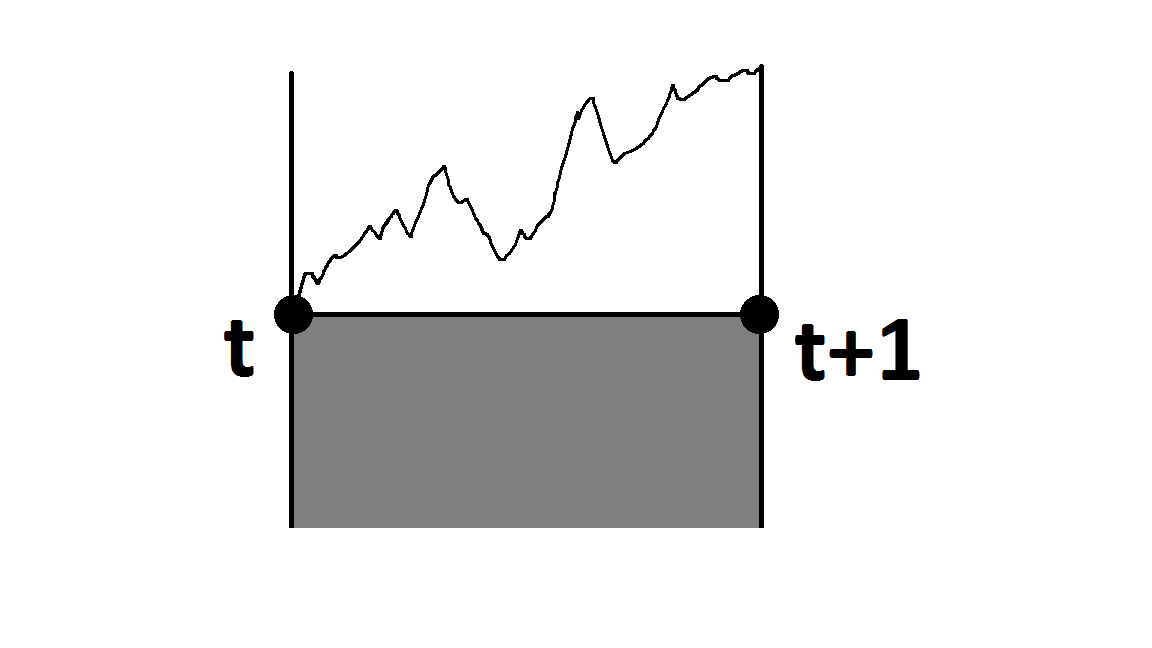
\includegraphics[scale=0.5]{Figure_1_ItoIntegral.png}\\
This is due to the quadratic variation. Because that much variance can accumulate overtime.\\
\\
% 2 figs
\\
Remarks:\\
$\rightarrow$ Ito integral is a limit of Riemannian sums when always taking left point of each interval.\\
$\rightarrow$ Taking left points means for each interval, you cannot see the future.\\
$\rightarrow$ 'equivalent' of Ito's Calculus: $(dB_t)=-dt$

\subsection{Adapted Process}
Definition:\\
$\Delta(t)$ is adapted to $X_t$ if $\forall t>=0$, $\Delta(t)$ depends only on $X_0\sim X_t$.(only dependent on the past)\\
Examples:\\
\begin{enumerate}
    \item $X_t$ is dependent on $X_t$
    \item $Y_t=X_{t+1}$ is not dependent on $X_t$.
    \item $\Delta(t)=min{X_t}$ is dependent on $X_t$.
    \item $T>0, \Delta(t)=mac{X_s}, (t<s<T)$ is not adaptable.
\end{enumerate}

\subsection{Theorem 1}
If $\Delta(t)$ is a process depends only on t, then:\\
\\
$X(t)=\int \Delta(t)dB_t$ has Normal Distribution.\\
\\Intuition: Sum of Normal Distributions(Random Variables) is Normal Distribution(Random Variable).\\

\subsection{Theorem 2: Ito Isometry}
If $X_t$ is adapted to $W_t$,\\
$$E[(\int_0^T X_t dW_t)^2]=E[\int_0^T X_t^2dt]$$
\\
Eg.(Quadratic Variation)\\
If $\Delta(t)=1$, then $E[B(t)^2]=t$.

\subsection{Theorem 3}
Question: When is Ito Integral a martingale?\\
\\
If $g(t,B_t)$ is adapted to $B_t$, then
$$\int g(t,B_t)dB_t$$
is a martingale as long as $\int\int g(t,B_t)^2<\infty$.\\
\\
\begin{itemize}
    \item $E[X_s|F_t]=X_t$ $\forall t<s$. (where $F_t=X_0 \sim X_t$)
%\any
%\subbrace for F_t{X_0\sim X_t}
    \item Eg.: If $dX_t=\mu(t,B_t)dt + \sigma(t,B_t)dBt$, then $X_t$ is a martingale if and only if $\mu=0$.
    \item For SDE: No Drift $\Leftrightarrow$ martingale.
\end{itemize}

\section{Lebesgue Integral}

$$\{E,X,\mu\}$$
$E$: set\\
$X$: $E$'s $\sigma$-algebra\\
$\mu$: measure\\
$$\int_X f d\mu$$
\begin{itemize}
    \item $X$: measurable space
    \item $\mu$: measure
\end{itemize}



\section{Log-Normal}
$$Y=ln(X) \sim N(\mu,\sigma^2)$$
$$X=exp(Y) \sim LN(\mu,\sigma^2)(Log-Normal)$$
$$E[e^x]=e^{E[x]+Var(x)}$$


\section{Black Scholes}
$$dS_t=\mu S_t dt + \sigma S_t dW_t$$
By Ito's Lemma
$$(ln(S))'=\frac{1}{S}, (ln(S))''=-\frac{1}{S^2}$$
$$dln(S_t)=(\mu-\frac{\sigma^2}{2})dt + \sigma dW_t$$
we get
$$\int_0^t dlnS_u = \int_0^t (\mu-\frac{1}{2}\sigma^2)du + \sigma\int_0^tdW_u$$
$$ln(S_t)-ln(S_0)=(\mu-\frac{1}{2}\sigma^2)t + \sigma W_t$$
$$S_t=S_0 e^{(\mu - \frac{1}{2}\sigma^2)+\sigma W_t}$$

\subsection{Black Scholes Equation}
$$V_t + \frac{1}{2}\sigma^2 S_t^2 V_{ss} +rS_t V_s - rV=0$$
proof:
$$dS_t=\mu S_t dt + \sigma S_t dt$$
$$V = V(S_t, t)$$

$$dV = (\mu S_t \frac{\partial V}{S_t} + \frac{\partial V}{dt} + \sigma^2 S_t^2 \frac{\partial^2 V}{\partial S_t^2})dt + \sigma S_t \frac{\partial V}{\partial S_t} dW_t$$
$$dV = (\mu S_t V_s + V_t + \sigma^2 S_t^2 V_{ss})dt + \sigma S_t V_s dW_t$$

Hedged portfolio:
\begin{align*} 
\Pi &= -V + \phi S_t,\quad \phi=\frac{\partial V}{\partial S_t}
\\
\Pi &= -V + V_s S_t
\\
d\Pi &= -dV + V_s dS_t
\\
d\Pi &= \Pi r d_t = (-V + V_s S_t)rdt
\\
-dV + V_s dS_t &= (-V + V_s S_t)rdt
\\
-V_t - \frac{1}{2}\sigma^2 S_t^2 V_{ss} &= r(-V + V_s S_t)
\\
0 &= V_t + \frac{1}{2}\sigma^2 S_t^2 V_{ss} +rS_t V_s - rV
\\
\end{align*} 

\subsection{Black Scholes Formula}


European call option price:

$$C(S_t,t)=Pr(S_T>K)(E[S_T|S_T>K]-K)$$
$$C(S_t,t)=N(d_1)S_t-N(d_2)Ke^{-r(T-t)}$$
$$d_1=\frac{1}{\sigma\sqrt{T-t}}[ln(\frac{S_t}{k}) + (r+\frac{\sigma^2}{2})(T-t)]$$
$$d_2=d_1-\sigma\sqrt{T-t}$$



\section{Doleans Dade exponential($\varepsilon$)}
(In the change of measure, we need to define a density process, during which we will need $\varepsilon$.)\\
Let $X_t$ be a measurable process adaptd to the filtration.\\
Doleans Dade exponential is the solution to:
$$dY_t=Y_tdX_t$$
which is the form of density process $dQ=\eta_tdP$.\\
Where $\eta_t$ is Radon-Nikodym derivative.
$$\varepsilon(X)_t=exp[X_t-\frac{1}{2}[X,X]_t]$$
$L$ is the inverse of $\varepsilon$.\\
$$W_t^*=W_t-[W,X]_t$$\\


\section{Change of Measure}
Question:\\
$B_t$: Brownian Motion without drift.\\
$\tilde{B_t}$: Brownian Motion with drift.\\
Can we switch between the probability distributions by a change of measure?\\
% ({\it \_2\_ChangeofMeasure.png})\\ not working
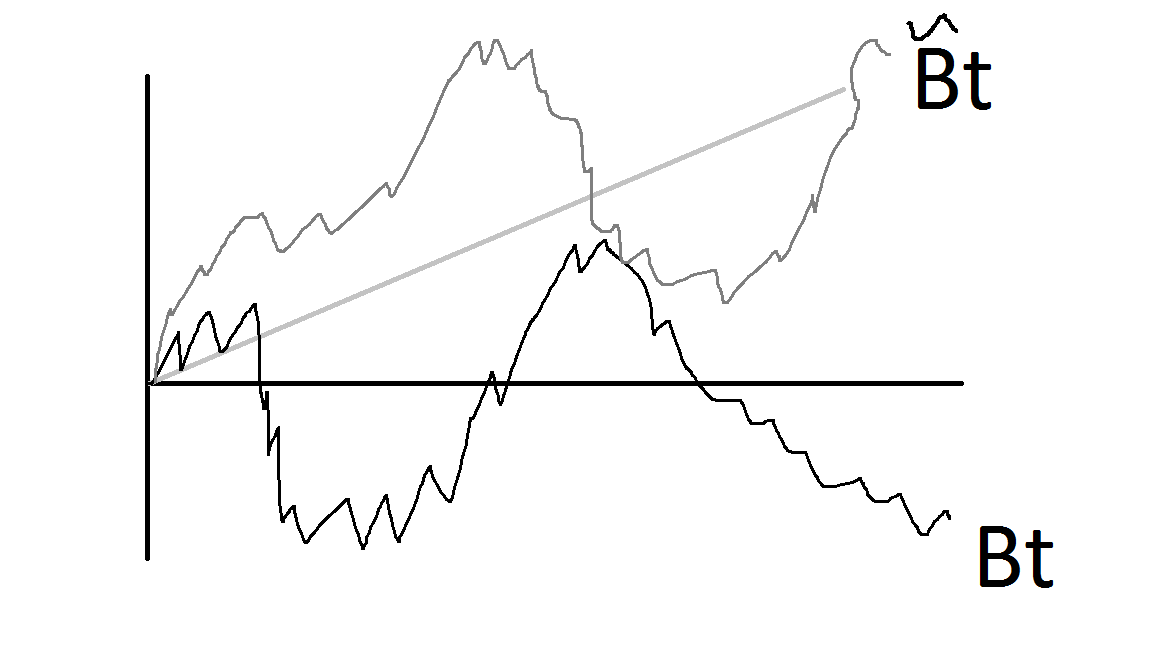
\includegraphics[scale=0.45]{Figure_2_ChangeofMeasure.png}\\
\\
$p(\omega)$: pdf by $B_t$.\\
$\tilde{p}(\omega)$: pdf by $\tilde{B_t}$.\\
$\exists Z=Z(\omega)\ s.t.\ p(\omega)=Z(\omega)\tilde{p}(\omega)$ ?\\
%\2 figs
\\
$(\Omega, P)$: Probaility distribution without drift.\\
$(\Omega, \tilde{P})$: Probability distribution with drift.\\
\\
Definition:\
$P$ and $\tilde{P}$ are equivalent if $P(A)>0\Leftrightarrow\tilde{P}(A)>0 \ (\forall A\in\Omega)$.
% \any

\subsection{Radon-Nikodym derivative}
$$\exists Z\ s.t.\ p(\omega)=Z(\omega)\tilde{p}(\omega)$$
if and only if $P$ and $\tilde{P}$ are equivalent.\\
$Z$: Radon-Nikodym derivative.

\subsection{Girsanov Theorem}
$P$: Probability distribution over $[0,T]^{\infty}$ defined by a BM with drift $\mu.$\\
(where $[0,T]^{\infty}$ means paths from 0 to T)\\
\\
$\tilde{P}$: Probability distribution over $[0,T]^{\infty}$ defined by a BM w/o drift $\mu.$\\
\\
The $P$ and $\tilde{P}$ are equivalent.
$$\Rightarrow Z(\omega)=\frac{d\tilde{P}}{dP}(\omega)=e^{-\mu W_T - \frac{1}{2}\mu^2 T}$$
$$\tilde{E}[V_t]=E[Z_t V_t]$$
\\
(where $\tilde{E}$ in Probability space $(\Omega,\tilde{P})$, $E$ in Probability space $(\Omega,P)$)


\section{Notation}
$S_T=S_0 e^{(\mu-\frac{1}{2}\sigma^2)T+\sigma W_T}$\\
$V_t$ : Value process\\
$\pi_{it}=\phi_{it} S_{it}$\\
$\phi$ : \# of shares
$\pi$ : dollar amount

\section{Mallivian Calculus}
$$M_v=E_v[F]$$
$$D_t M_v=E_v[D_tF]$$





\end{document}
